% !TEX program = xelatex
\documentclass[10pt,xcolor=svgnames]{beamer} %Beamer
%\usepackage{palatino} %font type
\usefonttheme{metropolis} %Type of slides
\usefonttheme[onlymath]{serif} %font type Mathematical expressions
\usetheme[progressbar=frametitle,titleformat frame=smallcaps,numbering=counter]{metropolis} %This adds a bar at the beginning of each section.
\useoutertheme[subsection=false]{miniframes} %Circles in the top of each frame, showing the slide of each section you are at

\usepackage{appendixnumberbeamer} %enumerate each slide without counting the appendix
\setbeamercolor{progress bar}{fg=Maroon!70!Coral} %These are the colours of the progress bar. Notice that the names used are the svgnames
\setbeamercolor{title separator}{fg=DarkSalmon} %This is the line colour in the title slide
\setbeamercolor{structure}{fg=black} %Colour of the text of structure, numbers, items, blah. Not the big text.
\setbeamercolor{normal text}{fg=black!87} %Colour of normal text
\setbeamercolor{alerted text}{fg=DarkRed!60!Gainsboro} %Color of the alert box
\setbeamercolor{example text}{fg=Maroon!70!Coral} %Colour of the Example block text


\setbeamercolor{palette primary}{bg=NavyBlue!50!DarkOliveGreen, fg=white} %These are the colours of the background. Being this the main combination and so one. 
\setbeamercolor{palette secondary}{bg=NavyBlue!50!DarkOliveGreen, fg=white}
\setbeamercolor{palette tertiary}{bg=NavyBlue!40!Black, fg=white}
\setbeamercolor{section in toc}{fg=NavyBlue!40!Black} %Color of the text in the table of contents (toc)
\setbeamercolor{background canvas}{bg=white}

%These next packages are the useful for Physics in general, you can add the extras here. 
\usepackage{amsmath,amssymb}
\usepackage{slashed}
\usepackage{cite}
\usepackage{relsize}
\usepackage[font=smaller, labelfont=bf, width=0.95\linewidth]{caption}
\usepackage{subcaption}
\usepackage{multicol}
\usepackage{booktabs}
\usepackage[scale=2]{ccicons}
\usepackage{pgfplots}
\usepgfplotslibrary{dateplot}
\usepackage{geometry}
\usepackage{xspace}

\usepackage{fouriernc}
\usepackage{MnSymbol}
\usepackage{tempora}

\newcommand{\themename}{\textbf{\textsc{bluetemp}\xspace}}%metropolis}}\xspace}

\title{Efficient directed scattering of XUV radiation using high-density spherical clusters}
\author[Name]{L.A. Litvinov, A.A. Andreev} %With inst, you can change the institution they belong
%\subtitle{Subtitle}
\institute[uni]{Department of General Physics I \\ Saint Petersburg State University}
\date{\today} %Here you can change the date
\titlegraphic{\vspace{5.5cm}\hfill
\includegraphics[scale=0.5]{../components/img/spbu_logo.png}} %You can modify the location of the logo by changing the command \vspace{}. 

\def \w{\omega}

% ------------------------- %

\def \eq{\begin{equation}}
\def \qe{\end{equation}}
\def \eqc{\begin{equation*}}
\def \cqe{\end{equation*}}

% ------------------------- %
\newcommand{\symbf}[2][bold symbol]{
    \mbox{\boldmath${#2}$}
}

% ------------------------- %

\newcommand{\indexbf}[2][bold index]{
    \mbox{\boldmath{#2}}
}

% ------------------------- %

\newcommand\shifthat[2]{%
  \stackengine{\Sstackgap}{$#2$}{\(\hspace{#1}\hat{}\)}{O}{l}{F}{T}{S}}

% ------------------------- %

\newcommand{\operator}[2][operator]{
    % \symbf{\hat{#2}} % works with default font
    % \hat{\textit{\textbf{#2}}} % italic bold style
    % bold style
    \if H#2\shifthat{0.5em}{#2}\else
    \if d#2\shifthat{0.49em}{#2}\else
    \if q#2\shifthat{0.35em}{#2}\else
    \if \mu#2\shifthat{0.35em}{#2}\else
    \shifthat{0.45em}{#2}
    \fi
    \fi
    \fi
    \fi
}

% ------------------------- %

\newcommand{\vectoperator}[2][operator]{
    % \symbf{\hat{#2}} % works with default font
    % \hat{\textit{\textbf{#2}}} % italic bold style
    % \symbf{\hat{#2}} % works with default font
    % \hat{\textit{\textbf{#2}}} % italic bold style
    % bold style
    \if d#2\shifthat{0.367em}{\textbf{#2}}\else
    \if m#2\shifthat{0.4em}{\textbf{#2}}\else
    \shifthat{0.275em}{\textbf{#2}}
    \fi
    \fi
}

% ------------------------- %

\newcommand{\vect}[3][vector]{
    \overrightarrow{#2_{#3}}
}

% ------------------------- %

\newcommand{\vectbf}[2][bold vector]{
    % \vect{\textit{\textbf{#2}}}
    \vect{\textbf{#2}}
}

% ------------------------- %

\newcommand{\pd}[3][empty]{
    \frac{\partial {#2}}{\partial {#3}}
}

% ------------------------- %

\newcommand{\func}[5][empty]{
    {#2}_{#3}^{#4} \left( {#5} \right)
}

% ------------------------- %

\newcommand{\underrel}[3][]{
    \mathrel{\mathop{#3}\limits_{
        \ifx c#1\relax\mathclap{#2}\else#2\fi
    }}
}

% ------------------------- %

\newcommand{\addimg}[5][anything]{
    \begin{figure}[H]{
        \center{\includegraphics[width={#5}]{{#1}} {#4}} % 0.8\textwidth
        \caption{#2}
        \label{#3}}
    \end{figure}
}

\begin{document}
{
\setbeamercolor{background canvas}{bg=NavyBlue!50!DarkOliveGreen, fg=white}
\setbeamercolor{normal text}{fg=white}
\maketitle
}%This is the colour of the first slide. bg= background and fg=foreground

\metroset{titleformat frame=smallcaps} %This changes the titles for small caps

% \begin{frame}{Outline}
%   \setbeamertemplate{section in toc}[sections numbered] %This is numbering the sections
%   \tableofcontents[hideallsubsections] %You can comment this line if you want to show the subsections in the table of contents
% \end{frame}

% \begin{frame}{Objectives}
% \underline{\textsc{Some text:}}
% \begin{small}
% This is some small Text. 
% \end{small}

% \metroset{block=fill}
% \begin{exampleblock}{\textsc{Example block}}
% \begin{itemize}
%     \item You know how to do itemize
%     \item Also here
% \end{itemize}
% \end{exampleblock}
% \end{frame}


\section{Introduction}

% 1024px-Siwiki.svg

% shit slide, need to replace in the future :/
\begin{frame}[fragile]{Mie theory}\
    \begin{center}
        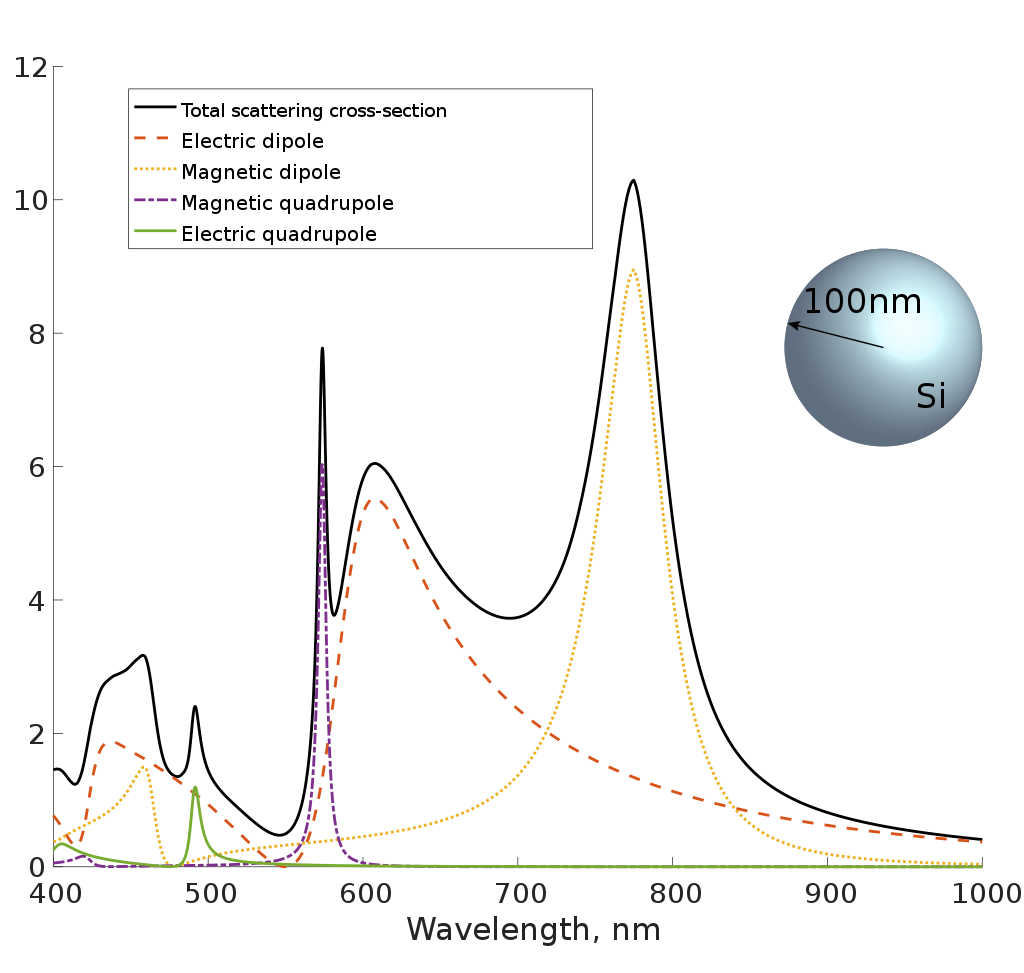
\includegraphics[width=0.6\textwidth]{../components/img/1024px-Siwiki.svg.png}
    \end{center}
\end{frame}

\begin{frame}[fragile]{XUV wavelength range}\
    \begin{center}
        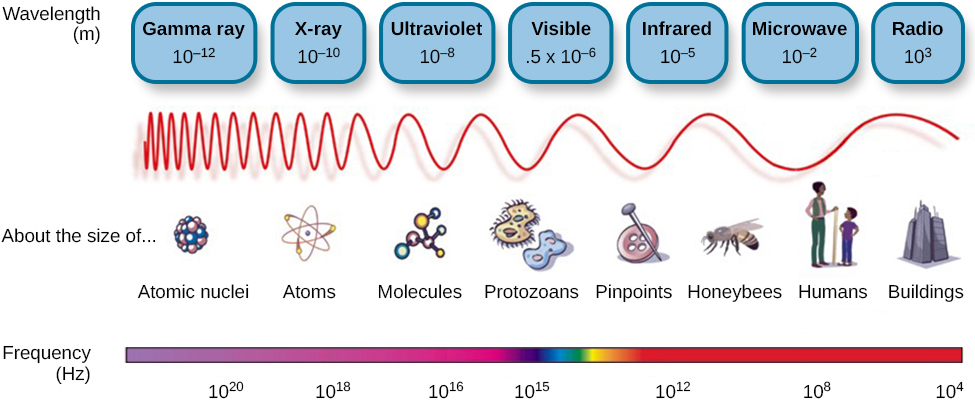
\includegraphics[width=1.\textwidth]{../components/img/CNX_Psych_05_02_Spectrum.jpg}
    \end{center}
\end{frame}

\begin{frame}[fragile]{Spherical vs cylindrical}
    \begin{center}
        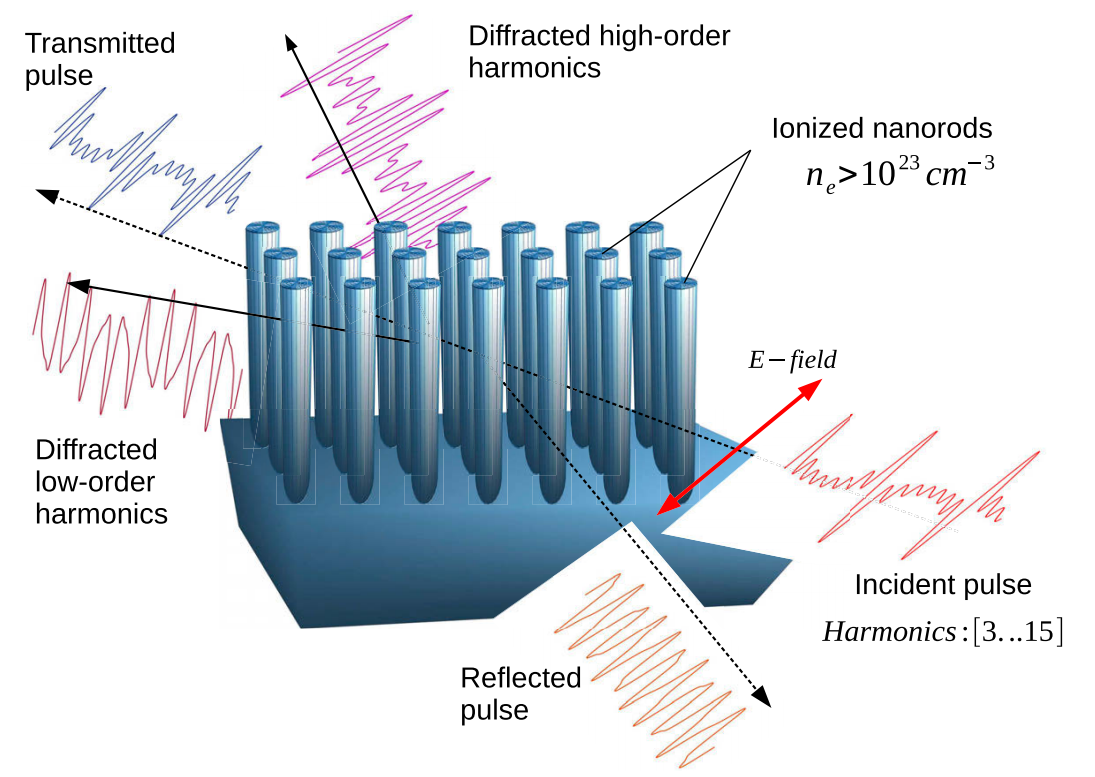
\includegraphics[width=0.8\textwidth]{../components/img/cyl_spsp.png}
    \end{center}
\end{frame}

% \begin{frame}[fragile]{Spherical vs cylindrical} %You can change fragile by standout
%     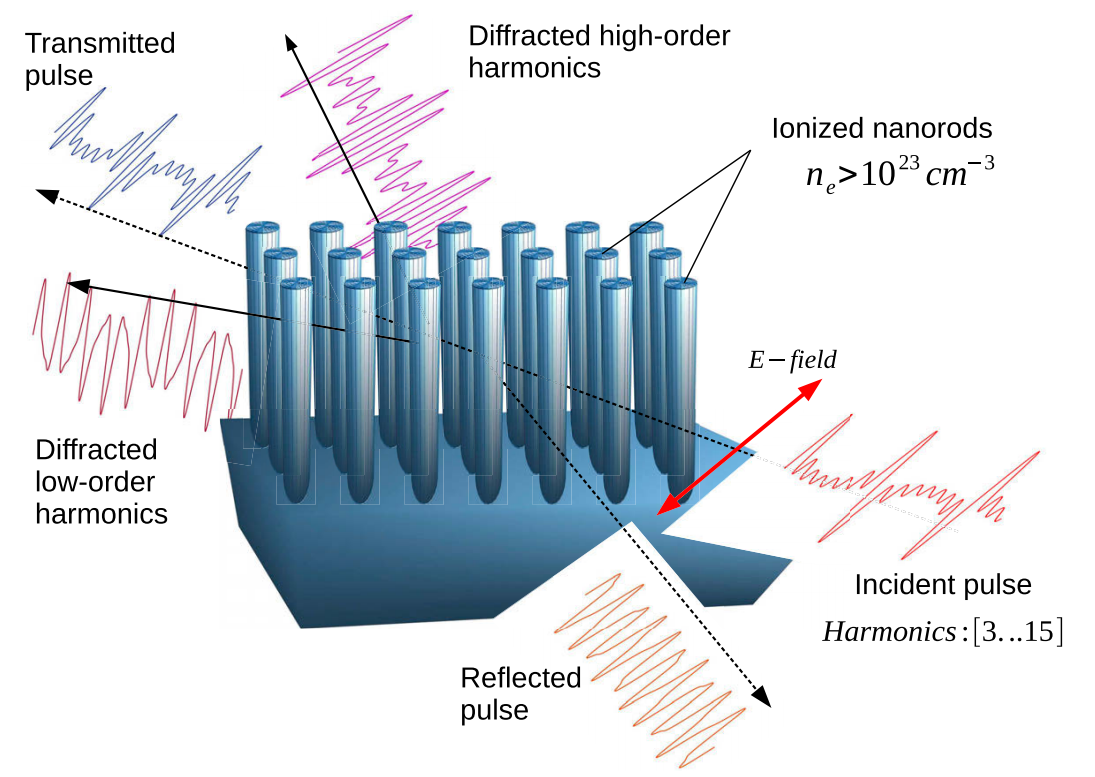
\includegraphics[width=0.8.\textwidth]{../components/img/cyl_spsp.png}
% \end{frame}

\begin{frame}[fragile]{Ionized cluster gas} %You can change fragile by standout
    \img[../components/img/cluster_gas_sheme]{Ionized cluster gas generation process.}{cluster_gas_sheme:image}{}{0.9\textwidth}
\end{frame}

\begin{frame}[fragile]{Interaction scheme} %You can change fragile by standout
    \img[../components/img/plasma_area2]{The plane of polarization is parallel to one of the faces of cubic region. The dimensions of spherical clusters are about a few nanometers, distance between them is at least wavelength. In general, the distribution of clusters within a cubic region is arbitrary without intersections.}{plasma_area1:image}{}{0.8\textwidth}
\end{frame}

\section{Base model}


\begin{frame}[fragile]{Base model scheme}
    \img[../components/img/single_sph_scheme]{Base model scheme.}{single_sph_scheme:image}{}{0.8\textwidth}
\end{frame}


\begin{frame}[fragile]{Zero-order approximation}
    \begin{figure}[H]
		(a)\:\subimg[../components/img/sph_base/sph_ka0.5_123]{0.6\textwidth}
		\\(b)\:\subimg[../components/img/sph_base/sph_ka1.5_123]{0.6\textwidth}
		\caption{Spherical harmonics coefficients. $ka = 0.5$ (a), $ka = 1.5$ (b) in zero-order approximation, $\beta_e = 0$.}
		\label{ab_asymp:image}
	\end{figure}
\end{frame}

\begin{frame}[fragile]{First-order approximation}
    \begin{figure}[H]
		(a)\:\subimg[../components/img/sph_base/sph_ka1.5_123]{0.6\textwidth}
        \\(b)\:\subimg[../components/img/sph_base/sph_ka1.5_123_1st]{0.6\textwidth}
		\caption{Spherical harmonics coefficients. $ka = 1.5$, (a) --- in zero-order approximation, (b) --- in first-order approximation, $\beta_e = 0$.}
		\label{ab_asymp2:image}
	\end{figure}
\end{frame}


\begin{frame}[fragile]{Resonance electron density}
    \img[../components/img/sph_base/nenc_123]{Resonance electron density depending on radius. Curves were calculated for resonant $m$ values, $\beta_e = 0$.}{nenc_123:image}{}{0.8\textwidth}
\end{frame}

\section{Single cluster}

\begin{frame}[fragile]{Considered cases}
    \begin{itemize}
        \item $ \lambda = \lambda_{L} = 830$ nm, $\lambda = \lambda_{10} = 83$ nm;
        \item $ka = 0.5, 0.7 \Rightarrow m_{0.5} = 1.635i$, $m_{0.7} = 1.851i$.
    \end{itemize}
\end{frame}

\begin{frame}[fragile]{$ka = 0.5~(a \approx 6.4~nm);~\lambda = \lambda_{L}=830~nm$}
    \begin{figure}[H]
        (a)\:\subimg[../components/img/mph/830nm_ka0.5_near]{0.42\textwidth}
        (b)\:\subimg[../components/img/mph/830nm_ka0.5_far]{0.42\textwidth}
        \caption{Laser harmonic scattering by a single cluster. $|\vectbf{E}{}|$ plotted in the plane of polarization, near-field (a) and far-field (b).}
        \label{1h_ka0.5:image}
    \end{figure}
\end{frame}

\begin{frame}[fragile]{$ka = 0.5~(a \approx 6.4~nm);~\lambda = \lambda_{10}=83~nm$}
    \begin{figure}[H]
        (a)\:\subimg[../components/img/mph/83nm_ka0.5_near_k_broken]{0.42\textwidth}
        (b)\:\subimg[../components/img/mph/83nm_ka0.5_far_k_broken]{0.42\textwidth}
        \caption{$10$-th harmonic scattering by a single cluster. $|\vectbf{E}{}|$ plotted in the plane of polarization, near-field (a) and far-field (b).}
        \label{10h_ka0.5:image}
    \end{figure}
\end{frame}

\begin{frame}[fragile]{$ka = 0.7~(a \approx 8.9~nm);~\lambda = \lambda_{L}=830~nm$}
    \begin{figure}[H]
        (a)\:\subimg[../components/img/mph/830nm_ka0.7_near]{0.42\textwidth}
        (b)\:\subimg[../components/img/mph/830nm_ka0.7_far]{0.42\textwidth}
        \caption{Laser harmonic scattering by a single cluster. $|\vectbf{E}{}|$ plotted in the plane of polarization, near-field (a) and far-field (b).}
        \label{1h_ka0.7:image}
    \end{figure}
\end{frame}

\begin{frame}[fragile]{$ka = 0.7~(a \approx 8.9~nm);~\lambda = \lambda_{10}=83~nm$}
    \begin{figure}[H]
        (a)\:\subimg[../components/img/mph/83nm_ka0.7_far_k_broken]{0.42\textwidth}
        (b)\:\subimg[../components/img/external/oe-28_screen]{0.46\textwidth}
        \caption{$10$-th harmonic scattering by a single cluster. $\lambda = \lambda_{L}$, $a \approx 8.9$~nm ($ka = 0.5$); $|\vectbf{E}{}|$ plotted in the plane of polarization far-field (a). For qualitative assessment field scattered by a single nanocylinder with the same $ka$ added (b) --- here the incident wave propagates from right to left (along negative $x$ axis direction), polarization is along $y$ axis.}
        \label{10h_ka0.7:image}
    \end{figure}
\end{frame}

\section{Multiple clusters}

\begin{frame}[fragile]{Configuration}
    \img[../components/img/scheme_lattice]{Model scheme, generalized target geometry.}{lattice_scheme:image}{}{0.9\textwidth}
\end{frame}

\begin{frame}[fragile]{$ka = 0.5~(a \approx 6.4~nm);~\lambda = \lambda_{10}=83~nm,~b = \lambda_{10}$}
    \begin{figure}[H]
        (a)\:\subimg[../components/img/celes/64sph_b83nm_l83nm_45deg_near]{0.4\textwidth}
        (b)\:\subimg[../components/img/celes/64sph_b83nm_l83nm_45deg_far]{0.4\textwidth}
        \caption{$10$-th harmonic scattering by multiple clusters. Incidence at $45^{\circ}$ angle; a --- near-field; b --- far-field.}
        \label{multi_sph_b1:image}
    \end{figure}
\end{frame}

\begin{frame}[fragile]{$ka = 0.5~(a \approx 6.4~nm);~\lambda = \lambda_{10}=83~nm,~b = 3\lambda_{10}$}
    \begin{figure}[H]
        (a)\:\subimg[../components/img/celes/64sph_b249nm_l83nm_30deg_near]{0.4\textwidth}
        (b)\:\subimg[../components/img/celes/64sph_b249nm_l83nm_30deg_far]{0.4\textwidth}
        \caption{$10$-th harmonic scattering by multiple clusters. Incidence at $30^{\circ}$ angle; a --- near-field; b --- far-field.}
        \label{multi_sph_b3:image}
    \end{figure}
\end{frame}


\begin{frame}[standout]{}
    \begin{center}
        {\Large Thanks for your attention}
    \end{center}
\end{frame}

\end{document}